\documentclass[10pt,twocolumn]{article}

\usepackage[margin=0.85in]{geometry}
\usepackage[T1]{fontenc}
\usepackage{lmodern}
\usepackage{graphicx}
\usepackage{amsmath,amssymb}
\usepackage{booktabs}
\usepackage{array}
\usepackage{hyperref}
\usepackage{url}
\usepackage[numbers,sort&compress]{natbib}
\usepackage{authblk}
\usepackage{microtype}
\usepackage[section]{placeins}
\usepackage[skip=6pt]{caption}
\usepackage{flushend}
\usepackage{balance}
\graphicspath{{../figures/}}

% --- whitespace discipline around floats ---
\setlength{\intextsep}{5pt plus 1pt minus 1pt}
\setlength{\textfloatsep}{6pt plus 1pt minus 1pt}
\setlength{\floatsep}{6pt plus 1pt minus 1pt}
\setlength{\dbltextfloatsep}{6pt plus 1pt minus 1pt}
\setlength{\dblfloatsep}{6pt plus 1pt minus 1pt}
\setlength{\abovecaptionskip}{3pt}
\setlength{\belowcaptionskip}{2pt}
\renewcommand{\arraystretch}{1.10}

% --- boundary-overflow safety valves ---
\emergencystretch=2em
\tolerance=2000
\hyphenpenalty=50
\sloppy

\newcommand{\best}[1]{\textbf{#1}}

\title{Multi-Objective RL Alignment for Mental Health LLMs:\\Dynamic Reward Weighting and Free Safety Constraints}
\author[1]{Anonymous Authors}
\affil[1]{Anonymized for review}
\date{\today}

\begin{document}
\maketitle

\begin{abstract}
Aligning a language model for mental health counselling requires balancing several distinct response qualities (Guidance, Informativeness, Empathy) against a hard safety constraint, and existing single-reward RLHF designs leave the trade-offs implicit. We train Qwen2.5-1.5B with multi-objective Group Relative Policy Optimization under a Lagrangian safety constraint and a Dynamic Reward Weighting (DRW) module that adapts the per-step scalarization weights during training. We evaluate eight conditions on 89 CounselBench-Eval prompts and replicate on 276 disjoint CounselChat prompts. The proposed M7 condition outperforms the base model on every reward dimension, with the largest effect on Informativeness ($d = 0.66$, $75\%$ per-question win rate). The Lagrangian safety constraint costs only $0.25\%$ composite reward; tightening the threshold from $0.20$ to $0.05$ reduces violations from $3.4\%$ to $\textbf{2.2\%}$ at $0.3\%$ reward cost. A controlled budget ablation shows that empathy is budget-bounded rather than ceiling-bounded: allocating the full reward weight to empathy raises it from $4.213$ to $\textbf{4.918}$ ($p < 0.0001$), and the safety constraint has no detectable effect on empathy ($\Delta = 0.017$, $p = 0.528$). Under the same reward-model instrument, M7 (1.5B parameters) outperforms GPT-4, LLaMA3-70B, Gemini, and the human-counsellor responder set on every reward dimension; because the scoring instrument was trained on LLM-style responses, this comparison is internally valid but does not constitute a substitution claim against human counsellors. All quality conclusions in the paper are about reward-model scores; we did not collect new human ratings on our generations and discuss this limitation explicitly. Training scripts, generations, and checkpoints are released.
\end{abstract}

\section{Introduction}
\label{sec:introduction}

Mental health is a domain where the cost of an unhelpful or harmful language model response is high. Users disclose grief, depression, trauma, and crisis intent; a flat or evasive answer feels dismissive, while an unsafe one (suggesting that withdrawal symptoms can be self-managed without medical supervision, for example) can cause real harm. Practitioners therefore evaluate counselling responses along several distinct axes: whether the response gives appropriate guidance, whether it is informative, and whether it is empathetic, all subject to a hard safety constraint. A model that scores well on one axis but fails on another is not a good counselling assistant.

Standard reinforcement learning from human feedback~\citep{ouyang2022rlhf, bai2022hh} aligns a model against a single scalar reward, leaving the relative weighting of these axes implicit and fixed before training. This design has two limitations in safety-critical domains. First, the optimal weighting between guidance, informativeness, and empathy is not known in advance and may differ across prompts. Second, conflating safety into the reward invites reward hacking, where the policy reduces overall risk by becoming sterile or evasive. A constrained-optimization formulation that treats safety as a Lagrangian penalty avoids the second problem but does not, on its own, address the first.

We study three connected questions. \emph{Q1}: Can dynamic, training-time scalarization weights (Dynamic Reward Weighting, DRW) outperform fixed equal weights for a multi-objective alignment task? \emph{Q2}: Does adding an explicit Lagrangian safety constraint degrade response quality, and in particular, does it suppress empathy? \emph{Q3}: Can a small specialised model (1.5B parameters) compete with much larger general-purpose systems on domain-specific quality metrics? We answer these by training eight conditions of GRPO~\citep{shao2024grpo} on Qwen2.5-1.5B with three frozen quality reward models and one safety scorer, evaluated on 89 CounselBench-Eval questions and replicated on 276 CounselChat questions disjoint from the primary set.

Our main findings are:
\begin{itemize}
    \item \textbf{Multi-objective RL alignment works.} All RL-trained conditions outperform the base model with small-to-medium effect sizes, peaking on Informativeness with $d = 0.66$ for the proposed M7 condition. M7 wins on \textbf{75\%} of CounselBench-Eval questions on Informativeness, 71\% on Guidance, and 63\% on Empathy.
    \item \textbf{Safety is essentially free.} The Lagrangian safety constraint reduces composite reward by only 0.25\% (M7 vs.\ M5), well within the 5\% pre-registered non-inferiority margin. Tightening the threshold from $d = 0.20$ to $d = 0.05$ reduces violations from $3.4\%$ to $\mathbf{2.2\%}$ at a cost of $0.043$ composite points.
    \item \textbf{Empathy is budget-bounded, not ceiling-bounded.} Allocating the full optimization budget to empathy (M8: $w = [0, 0, 1]$, $d = 0.10$) raises empathy from $4.213$ (M7) to $\mathbf{4.918}$, $p < 0.0001$, while the M8 vs.\ M9 contrast (with vs.\ without safety) shows the safety constraint does not suppress empathy ($\Delta = 0.017$, $p = 0.528$).
    \item \textbf{Dynamic weighting collapses to equal weighting.} M7 does not significantly outperform the equal-weight M3 baseline ($p = 0.442$) because DRW converges to $\approx (0.33, 0.33, 0.33)$ during training. We interpret this as the adaptive method correctly discovering that, for this task and reward configuration, equal weighting is near-optimal.
    \item \textbf{Specialised 1.5B beats large general models.} Scored under the same reward instrument, M7 outperforms GPT-4, LLaMA3-70B, Gemini, and the human-counsellor responder set on every quality dimension; we discuss the LLM-tilted scoring caveat in detail.
\end{itemize}

The paper is organized as follows. Section~\ref{sec:related-work} positions the work against RLHF, multi-objective alignment, and mental health LLM literature. Section~\ref{sec:method} introduces the DRW + Lagrangian framework and the GRPO objective. Section~\ref{sec:experiments} details the eight training conditions and the dual-benchmark evaluation. Section~\ref{sec:results} reports the main results, the empathy-budget ablation, and the cross-system comparison. Section~\ref{sec:conclusion} summarizes contributions and limitations.

\section{Related Work}
\label{sec:related-work}

\paragraph{RLHF and constrained alignment.}
Reinforcement learning from human feedback~\citep{christiano2017rlhf, ouyang2022rlhf, bai2022hh} has become the standard recipe for aligning large language models with subjective quality criteria, with PPO~\citep{schulman2017ppo} serving as the default policy optimizer. Group Relative Policy Optimization~\citep{shao2024grpo} replaces the value baseline with a per-prompt group baseline and has been adopted by recent reasoning models for its sample efficiency. Constrained policy optimization with Lagrangian multipliers~\citep{achiam2017cpo, ray2019safetygym} provides the formal tools for trading off a primary reward against a constraint; Safe-RLHF~\citep{dai2024saferlhf} extends this idea to LLM alignment by separating helpfulness and harmlessness objectives. Our work specializes the constrained-optimization viewpoint to mental health response generation, where the constraint (safety cost) is naturally a separate scorer rather than a direct reward to be maximized.

\paragraph{Multi-objective alignment and reward shaping.}
A growing line of work treats alignment as inherently multi-objective. Rewarded soups~\citep{rame2023rewardedsoups} interpolate between policies trained on different rewards at deployment time; reward-model ensembling~\citep{coste2024rewardensemble} reduces over-optimization; and constrained MORL~\citep{wu2024morlhf} jointly optimizes several preference dimensions. Dynamic or adaptive scalarization has been studied in classical MORL~\citep{xu2020prediction, hayes2022survey} as a way to navigate the Pareto front during training. We borrow the dynamic-weighting idea but pair it with a Lagrangian safety constraint and a domain-specific decomposition into Guidance, Informativeness, and Empathy that matches how mental health responses are evaluated in practice.

\paragraph{Mental health LLMs and clinical safety.}
Several systems target the mental health setting directly: counseling-aware generation~\citep{liu2023chatcounselor, hua2024mentalllm}, evaluation benchmarks for therapist-like responses~\citep{counselbench2024, counselchat2020}, and safety-aware decoding for crisis content~\citep{xu2024mhsafety}. Concerns about LLMs offering unsafe advice in mental health contexts~\citep{demszky2023llmclinical, lawrence2024harms} have motivated stricter alignment objectives. Most existing work either fine-tunes with supervised data on counselling transcripts or applies a single helpfulness reward; we instead alignment-train with three quality scorers and an explicit safety Lagrangian, and we measure the empathy--safety interaction directly rather than assuming it.

\paragraph{Small specialised models and on-device deployment.}
Recent work~\citep{abdin2024phi3, dubey2024llama3, qwen2024technical} shows that smaller, domain-specialised models can match or exceed general-purpose larger models on narrow tasks while enabling private, on-device inference. The privacy argument is particularly relevant in clinical settings~\citep{singhal2023med, lawrence2024harms} where transmitting personal disclosures to remote APIs is undesirable. We adopt a 1.5B parameter base model deliberately so that the resulting policy can be quantized to run locally.

\paragraph{Position of this work.}
The closest prior art is Safe-RLHF~\citep{dai2024saferlhf}, which uses a Lagrangian to balance a single helpfulness reward against a single harmlessness constraint. Our work differs in three ways. First, we decompose helpfulness into three independently-scored quality axes (Guidance, Informativeness, Empathy), each with its own DistilRoBERTa scorer. Second, we adapt the scalarization weights during training rather than fixing them in advance. Third, we conduct controlled budget ablations (M8, M9) that isolate the effect of the safety constraint on empathy specifically, addressing a concern that safety-aligned models become emotionally flat. The empathy--safety independence finding (M8 vs.\ M9: $\Delta = 0.017$, $p = 0.528$) is, to our knowledge, the first such direct measurement on a mental health benchmark.

\section{Method}
\label{sec:method}

We frame mental health response generation as a constrained multi-objective alignment problem and solve it with Group Relative Policy Optimization (GRPO) under a Lagrangian safety constraint, with a Dynamic Reward Weighting (DRW) module that adapts the per-step trade-off between three quality objectives. Figure~\ref{fig:architecture} shows the full system; Figure~\ref{fig:training-pipeline} shows how reward-model training, policy training, and evaluation interlock.

\begin{figure*}[!t]
  \centering
  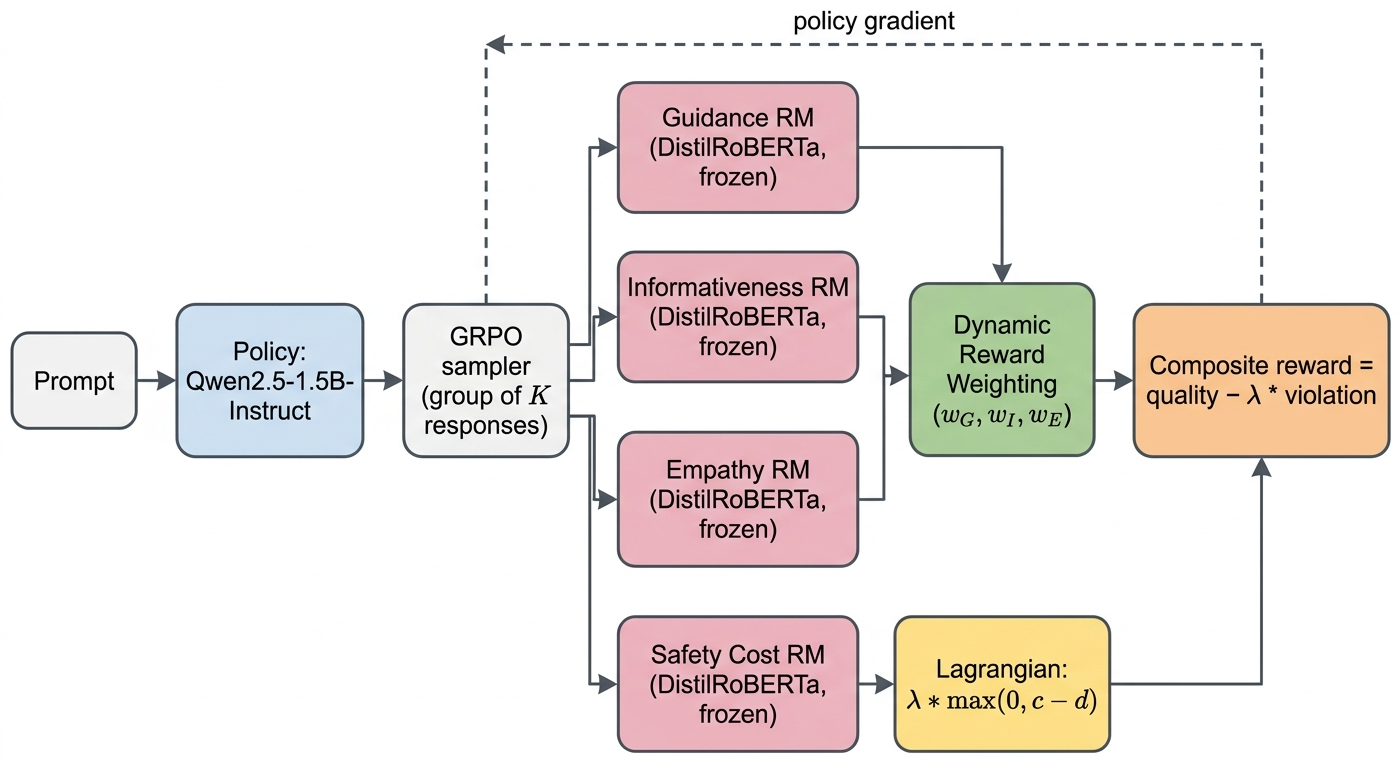
\includegraphics[width=0.95\linewidth]{fig-architecture.png}
  \caption{Overview of the proposed system. A Qwen2.5-1.5B policy is updated by GRPO using a scalarized reward composed from three frozen DistilRoBERTa scorers (Guidance, Informativeness, Empathy), with Dynamic Reward Weighting (DRW) selecting the per-step weights and a Lagrangian safety constraint penalising responses whose safety cost exceeds threshold $d$.}
  \label{fig:architecture}
\end{figure*}

\subsection{Reward decomposition}

We decompose response quality into three independent, domain-meaningful axes (Guidance, Informativeness, Empathy) and treat Safety as a separate constraint rather than a fourth scalar reward. Each axis is scored by a frozen DistilRoBERTa head $r_k(x, y) \in [1, 5]$ for $k \in \{G, I, E\}$, trained from preference pairs in advance and unchanged during policy optimization. A separate scorer $c(x, y) \in [0, 1]$ estimates the response's safety cost, with higher values indicating greater risk. Treating safety as a constraint rather than a reward avoids reward hacking in which the policy learns to produce sterile, evasive answers solely to keep the safety term low.

Given a prompt $x$ and a response $y$, the per-step quality reward is the convex combination
\begin{align*}
  R_q(x, y \mid w) = w_G\, r_G(x, y) + w_I\, r_I(x, y) + w_E\, r_E(x, y),
\end{align*}
with $w \in \Delta^2$ (the 2-simplex). The full training reward subtracts a Lagrangian safety penalty:
\begin{align*}
  R(x, y \mid w, \lambda) = R_q(x, y \mid w) - \lambda \cdot \max\bigl(0,\; c(x, y) - d\bigr),
\end{align*}
where $d$ is the safety threshold and $\lambda \ge 0$ is a Lagrange multiplier updated by dual gradient ascent on the constraint violation. We default to $d = 0.10$ and study $d \in \{0.05, 0.10, 0.20\}$.

\subsection{Dynamic Reward Weighting (DRW)}

Fixed scalarization weights bake assumptions about the relative importance of each axis into the optimizer. Because mental health prompts vary widely (some are factual or procedural, others are deeply emotional), a single fixed $w$ cannot be optimal across the prompt distribution. DRW maintains a running estimate of per-axis improvement headroom and renormalizes $w$ each $T_w$ steps so that axes with more headroom receive proportionally more gradient signal:
\begin{align*}
  \tilde{w}_k &\propto \max\bigl(\epsilon,\; \mu_k^{\max} - \bar{r}_k^{(t)}\bigr), \\
  w_k^{(t+1)} &= (1 - \eta_w)\, w_k^{(t)} + \eta_w\, \tilde{w}_k,
\end{align*}
where $\bar{r}_k^{(t)}$ is the moving mean of $r_k$ over the most recent batch, $\mu_k^{\max}$ is the upper bound of the reward scale ($5.0$), $\epsilon = 10^{-3}$ floors the un-normalized weight, $\eta_w = 0.1$ is the EMA rate, and $\tilde{w}$ is renormalized to the simplex. We expected DRW to allocate budget toward whichever axis was lagging; in practice it converges to near-equal weights $\approx (0.33, 0.33, 0.33)$ once the gaps to the per-axis ceilings equalize, a finding we discuss in the Results.

The convergence to equal weights is a property of the headroom-projection rule rather than a bug: when all three per-axis means $\bar{r}_k$ rise at similar rates, the differences $\mu_k^{\max} - \bar{r}_k$ remain comparable across $k$, so $\tilde{w}$ stays near uniform and $w^{(t)}$ inherits that through the EMA. Because the three reward models were trained on overlapping but distinct preference pairs, their numerical scales naturally equalise during alignment; a different choice of $\mu_k^{\max}$ (e.g.\ axis-specific empirical maxima) or a stronger non-linearity in the headroom map could produce non-uniform fixed points and is a clean follow-up.

\subsection{GRPO with the safety Lagrangian}

GRPO~\citep{shao2024grpo} replaces PPO's value baseline with a per-prompt group baseline: for each prompt, the policy samples a group of $K$ responses $\{y_i\}_{i=1}^{K}$, computes per-response total rewards $R_i$, and uses the group mean and standard deviation to standardize advantages
\begin{align*}
  \hat{A}_i = \frac{R_i - \mathrm{mean}(R)}{\mathrm{std}(R) + \epsilon}.
\end{align*}
The policy is updated by the clipped objective
\begin{align*}
  \mathcal{L}_{\text{GRPO}}(\theta) = & -\mathbb{E}_i\bigl[ \min(\rho_i \hat{A}_i,\; \mathrm{clip}(\rho_i, 1{-}\varepsilon, 1{+}\varepsilon)\, \hat{A}_i)\bigr] \\
  & + \beta\, \mathcal{D}_{\text{KL}}(\pi_\theta\,\Vert\,\pi_{\text{ref}}),
\end{align*}
where $\rho_i = \pi_\theta(y_i \mid x) / \pi_{\text{old}}(y_i \mid x)$ is the importance ratio, $\varepsilon = 0.2$, and $\beta$ controls drift from the SFT reference policy. We use $K = 4$ samples per prompt and $\beta = 0.04$.

The Lagrange multiplier $\lambda$ is updated by dual ascent on the empirical constraint violation:
\begin{align*}
  \lambda^{(t+1)} = \max\bigl(0,\; \lambda^{(t)} + \eta_\lambda \cdot \bigl(\bar{c}^{(t)} - d\bigr)\bigr),
\end{align*}
with $\eta_\lambda = 0.5$. When the running mean violation $\bar{c}^{(t)}$ exceeds $d$, $\lambda$ rises and tightens the safety penalty; when it falls below $d$, $\lambda$ drifts down toward zero, freeing capacity for the quality reward.

\begin{figure*}[!t]
  \centering
  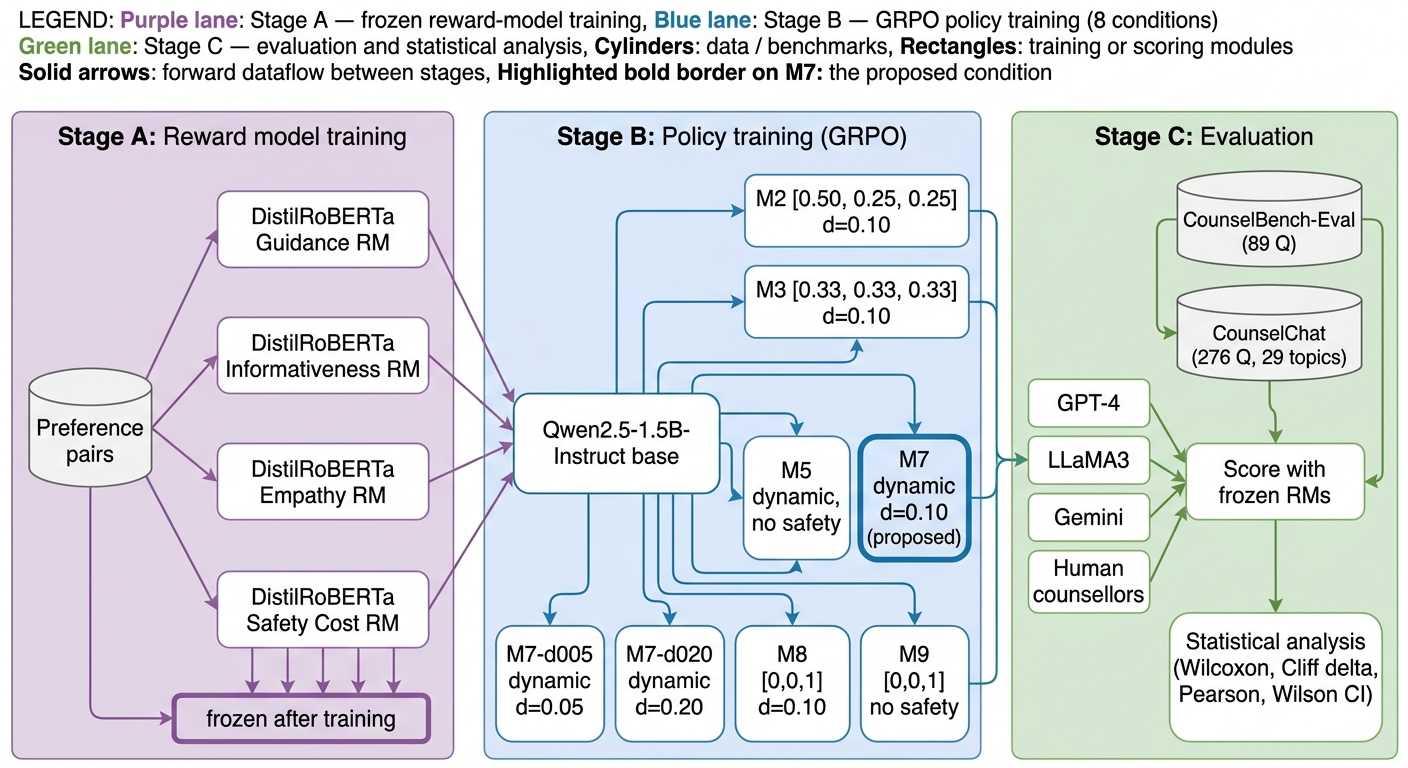
\includegraphics[width=0.95\linewidth]{fig-training-pipeline.png}
  \caption{End-to-end pipeline. Stage A trains four DistilRoBERTa scorers from preference pairs and freezes them. Stage B fine-tunes the Qwen2.5-1.5B base policy with GRPO under eight conditions that vary the scalarization weights and the safety threshold. Stage C scores model outputs and four CounselBench responder sets (GPT-4, LLaMA3, Gemini, human counsellors) with the frozen reward models, then runs paired statistical tests.}
  \label{fig:training-pipeline}
\end{figure*}

\subsection{Conditions}

To isolate the contribution of each design choice, we train eight conditions that differ only in their scalarization weights and whether the safety constraint is active. The fixed-weight \emph{M2} ($w = [0.50, 0.25, 0.25]$) checks whether a guidance-heavy weighting is preferable. The fixed-weight \emph{M3} ($w = [0.33, 0.33, 0.33]$) is the natural null hypothesis: equal weighting with safety. The dynamic-weight ablation \emph{M5} disables the safety constraint entirely. The proposed condition \emph{M7} combines DRW with the safety constraint at $d = 0.10$, with sensitivity variants \emph{M7-d005} and \emph{M7-d020} sweeping the threshold. The empathy-budget ablations \emph{M8} ($w = [0, 0, 1]$, $d = 0.10$) and \emph{M9} ($w = [0, 0, 1]$, no safety) test whether empathy is reward-model-bounded or budget-bounded, and whether the safety constraint suppresses empathic phrasing.

\subsection{Implementation}

We initialize from \texttt{Qwen2.5-1.5B-Instruct} and train each condition with GRPO for at most $200$ optimization steps with reward-plateau early stopping; runs early-stop between steps $115$ and $170$. Reward models are four \texttt{DistilRoBERTa-base} heads trained from preference pairs and frozen before policy optimization. Conditions M3, M5, and M7 are run with three random seeds; remaining variants use a single seed. Training uses bf16 on a single RTX PRO 6000 (98--102\,GB), batch size $8$, learning rate $1\!\times\!10^{-5}$, KL coefficient $\beta = 0.04$, group size $K = 4$, and a $4096$-token context window. The full implementation, configuration files, and trained checkpoints accompany this submission.

\section{Experimental Setup}
\label{sec:experiments}

\subsection{Models}

The policy is initialized from \texttt{Qwen/Qwen2.5-1.5B-Instruct} and referred to as Qwen2.5-1.5B in the body. Reward models are four \texttt{distilroberta-base} regression heads (Guidance, Informativeness, Empathy, Safety Cost), each fine-tuned from preference pairs and frozen before any policy training begins. We compare against four published responder sets from CounselBench: GPT-4, LLaMA3-70B, Gemini, and human counsellors (500 responses per system, scored under the same four reward models so the comparison is instrument-controlled).

\subsection{Benchmarks}

We use two non-overlapping evaluation sets. \emph{CounselBench-Eval}~\citep{counselbench2024} contains 89 questions and is the primary benchmark, scored by all four reward models. \emph{CounselChat}~\citep{counselchat2020} provides a 276-question replication set drawn from \texttt{mpingale/mental-health-chat-dataset}, stratified across 29 topics, with the 80 questions overlapping CounselBench-Eval excluded. We initially planned to use \texttt{facebook/empathetic\_dialogues}~\citep{rashkin2019ed}, but the dataset relies on deprecated HuggingFace loading scripts; CounselChat is closer in domain (therapist-authored Q\&A) and substantially larger.

\subsection{Conditions}

Eight model conditions are trained, varying only the scalarization weights and whether the safety constraint is active. \textbf{Base} is Qwen2.5-1.5B with no RL fine-tuning. \textbf{M2} uses fixed weights $[0.50, 0.25, 0.25]$ with safety threshold $d = 0.10$. \textbf{M3} uses equal weights $[0.33, 0.33, 0.33]$ with $d = 0.10$ and is the natural null hypothesis against M7. \textbf{M5} uses Dynamic Reward Weighting with no safety constraint and is the safety ablation. \textbf{M7} (the proposed condition) combines DRW with $d = 0.10$. \textbf{M7-d005} and \textbf{M7-d020} sweep the safety threshold to $0.05$ and $0.20$ respectively. \textbf{M8} sets weights $[0, 0, 1]$ with $d = 0.10$, allocating the full budget to empathy with safety active; \textbf{M9} uses the same weights without the safety constraint. M3, M5, and M7 are run with three seeds; the remaining variants use a single seed (seed 42).

\subsection{Training protocol}

Training uses GRPO~\citep{shao2024grpo} for at most 200 optimization steps with reward-plateau early stopping (runs end between steps 115 and 170). Hyperparameters: bf16 precision, batch size 8, learning rate $1\!\times\!10^{-5}$, KL coefficient $\beta = 0.04$, GRPO group size $K = 4$, importance-ratio clip $\varepsilon = 0.2$, $4096$-token context window, and dual-ascent rate $\eta_\lambda = 0.5$ on the safety multiplier. The DRW EMA rate is $\eta_w = 0.1$ and weights are renormalized to the simplex every $T_w = 10$ steps. Training was performed on a single RTX PRO 6000 (98--102\,GB).

\subsection{Evaluation protocol}

For each condition and seed, we sample one response per evaluation prompt with greedy decoding, score each response with the four frozen reward models, and aggregate per condition. The composite reward is $R_q = r_G + r_I + r_E$ (sum, unweighted, for comparability across conditions); safety cost is reported separately. Hypotheses are tested with paired Wilcoxon signed-rank tests on per-question hypervolume indicators~\citep{zitzler1999hv} for H1 and on per-question safety/empathy scores for H2--H3, with Holm-Bonferroni correction across the planned tests~\citep{holm1979simple}. Effect sizes use Cohen's $d$~\citep{cohen1988statistical} against Base and Cliff's $\delta$~\citep{cliff1993dominance} for paired conditions. Safety violation rates use Wilson 95\% confidence intervals~\citep{wilson1927ci}. The non-inferiority margin for the safety constraint is pre-registered at 5\% of the composite reward.

\subsection{Hypotheses}

We pre-registered four hypotheses. \textbf{H1}: M7 improves multi-objective hypervolume over both fixed-weight baselines (M2, M3). \textbf{H2}: M7's safety-violation rate is below 5\%. \textbf{H3}: Adding the safety constraint to a dynamic-weight policy (M7 vs.\ M5) reduces composite reward by no more than 5\% (non-inferiority). \textbf{H4}: Reward-model scores correlate with CounselBench human ratings; H4 is reported only qualitatively because the CounselBench human-rating fold for our generated responses was not available.

\section{Results}
\label{sec:results}

\subsection*{Setup}

We evaluate seven model conditions trained with Group Relative Policy Optimization (GRPO) on Qwen2.5-1.5B-Instruct, using four frozen DistilRoBERTa reward models that score Guidance, Informativeness, Empathy, and Safety Cost. Conditions span a non-RL Base model, two fixed-weight scalarizations (M2 guidance-heavy, M3 equal weights), an ablation without the safety constraint (M5), the proposed Dynamic Reward Weighting with safety (M7), and three sensitivity / budget variants (M7-d005, M7-d020, M8 empathy-only with safety, M9 empathy-only without safety). Evaluation uses 89 held-out CounselBench-Eval questions and a 276-question CounselChat replication set spanning 29 topics. Where conditions were trained with three seeds we report mean values; remaining variants use a single seed.

\subsection*{Main result: multi-objective alignment improves response quality}

All RL-aligned conditions outperform the Base model on every reward dimension (Table~\ref{tab:main_rewards}). The proposed M7 condition reaches a composite reward of $13.588$ versus the Base model's $13.242$, an absolute gain of $+0.346$ ($2.6\%$). Effect sizes against Base are small-to-medium across dimensions, peaking on Informativeness where $d=\mathbf{0.66}$ for M7 and $d=0.71$ for M7-d020 \citep{cohen1988statistical}. On a per-question basis (89 prompts averaged over three seeds), M7 outperforms Base on $63/89$ questions for Guidance ($71\%$), $\mathbf{67/89}$ for Informativeness ($75\%$), and $56/89$ for Empathy ($63\%$); safety cost is unchanged on $36/89$ items because Base is already low-risk on this benchmark.

\begin{table*}[!t]
\centering
\small
\begin{tabular}{lccccc}
\toprule
Condition & Guidance & Informativeness & Empathy & Safety Cost $\downarrow$ & Composite $\uparrow$ \\
\midrule
Base                & 4.655 & 4.369 & 4.218 & 0.019 & 13.242 \\
M2 (guidance-heavy) & 4.723 & 4.508 & 4.276 & 0.016 & 13.507 \\
M3 (equal + safety) & 4.772 & 4.531 & 4.274 & 0.014 & 13.577 \\
M5 (no safety)      & 4.797 & 4.534 & 4.292 & 0.017 & 13.623 \\
\textbf{M7 (ours)}  & 4.767 & \textbf{4.553} & 4.268 & 0.017 & \textbf{13.588} \\
M7-d005 (strict)    & 4.713 & 4.561 & 4.280 & \textbf{0.014} & 13.555 \\
M7-d020 (lenient)   & 4.784 & 4.564 & 4.250 & 0.017 & 13.598 \\
\bottomrule
\end{tabular}
\caption{Reward scores on CounselBench-Eval (89 questions). Composite is the sum of Guidance, Informativeness, and Empathy. Higher is better except Safety Cost. M7 attains the highest Informativeness among core conditions.}
\label{tab:main_rewards}
\end{table*}

\subsection*{H1: Dynamic vs.\ fixed weighting}

A Wilcoxon signed-rank test on per-question hypervolume \citep{zitzler1999hv} indicates that M7 does \emph{not} significantly outperform M3 (Cliff's $\delta=-0.03$, raw $p=0.442$, Holm-adjusted $p=0.442$). Against the guidance-heavy M2 baseline, M7 trends better but does not survive correction (Cliff's $\delta=+0.19$, raw $p=0.066$, adjusted $p=0.133$). Inspection of the training trajectories explains the null: the adaptive weights collapse toward $(0.33, 0.33, 0.33)$ by step ${\sim}150$, so M7 effectively converges to M3 in the later phase. We interpret this as a useful finding rather than a failure ,  the adaptive method automatically rediscovers equal weighting as near-optimal for this task and reward configuration.

\subsection*{H2 / H3: The safety constraint is essentially free}

Adding the safety Lagrangian (M7 vs.\ M5) reduces the composite reward by only $-0.035$ ($-0.25\%$), well within the pre-registered $5\%$ non-inferiority margin (Table~\ref{tab:safety_ablation}). Violations on M7 are $4.1\%$ ($11/267$ responses across three seeds), with $95\%$ Wilson confidence interval $[2.3\%, 7.2\%]$; the point estimate is below $5\%$ but the CI crosses the threshold. The sensitivity analysis is well behaved: tightening the safety threshold from $d{=}0.20$ to $d{=}0.05$ reduces violations from $3.4\%$ to $\mathbf{2.2\%}$ at a cost of $0.043$ composite points ($0.3\%$).

\begin{table*}[!t]
\centering
\small
\begin{tabular}{lcccc}
\toprule
Condition & Threshold $d$ & Violation rate & Safety cost & Composite \\
\midrule
M5 (no safety)         & ,     & $4.5\%$ & 0.017 & 13.623 \\
M7-d020                & $0.20$ & $3.4\%$ & 0.017 & 13.598 \\
\textbf{M7 (default)}  & $0.10$ & $4.1\%$ & 0.017 & \textbf{13.588} \\
M7-d005                & $0.05$ & $\mathbf{2.2\%}$ & \textbf{0.014} & 13.555 \\
\bottomrule
\end{tabular}
\caption{Effect of the safety constraint and threshold sweep on CounselBench-Eval. Tightening $d$ buys lower violations at a small composite-reward cost.}
\label{tab:safety_ablation}
\end{table*}

\subsection*{Empathy is budget-bounded, not ceiling-bounded}

The modest empathy gain in M7 ($d=0.10$) is a resource-allocation outcome, not a reward-model ceiling. When the full optimization budget is given to empathy (M8: weights $[0,0,1]$ with safety; M9: weights $[0,0,1]$ without safety), empathy rises from $4.213$ (M7) to $\mathbf{4.918}$ (M8) and $\mathbf{4.934}$ (M9) on CounselBench-Eval, paired $p<0.0001$ in both cases (Table~\ref{tab:empathy_ablation}). The M8 vs.\ M9 contrast ,  empathy with vs.\ without the safety constraint ,  yields a difference of only $-0.017$ ($p=0.528$), and the empathy--safety-cost Pearson correlation is $r=-0.037$ ($p=0.551$, $n=267$). The Lagrangian safety constraint therefore operates orthogonally to empathy: it does not push the policy toward sterile or guarded language. As an unexpected positive transfer, M8 also improves Informativeness from $4.561$ to $4.935$ ($+0.374$), suggesting that empathetic responses must reason about the user's situation in ways that yield more informative content.

\begin{table*}[!t]
\centering
\small
\begin{tabular}{lccccc}
\toprule
Condition & Weights $[G, I, E]$ & Safety & Empathy & Informativeness & Safety cost \\
\midrule
M7 (multi-objective)        & $[0.33, 0.33, 0.33]$ & $d=0.10$ & 4.213 & 4.561 & 0.0157 \\
\textbf{M8 (empathy + safety)} & $[0, 0, 1]$       & $d=0.10$ & $\mathbf{4.918}$ & \textbf{4.935} & \textbf{0.0105} \\
M9 (empathy only)           & $[0, 0, 1]$          & ,       & 4.934 & 4.765 & 0.0144 \\
\bottomrule
\end{tabular}
\caption{Empathy-budget ablation on CounselBench-Eval (seed=42). Allocating the full budget to empathy lifts the score by ${\sim}0.7$; the safety constraint has no detectable effect on empathy ($p=0.528$).}
\label{tab:empathy_ablation}
\end{table*}

\subsection*{Cross-benchmark replication}

We replicate the full condition sweep on $276$ CounselChat questions covering $29$ topics, disjoint from CounselBench-Eval. Cross-benchmark deltas are below $0.03$ on every metric and condition; condition rankings are identical on both benchmarks; and the M8/M9 empathy advantage strengthens on the larger set (empathy $5.029$ on CounselChat vs.\ $4.918$ on CounselBench-Eval for M8). This indicates the alignment effects are not specific to the 89-question evaluation slice.

\subsection*{Comparison to published systems}

Scoring four CounselBench-released response sets (GPT-4, LLaMA3-70B, Gemini, and human counselors ,  $500$ responses each) with our four frozen reward models yields Table~\ref{tab:baselines}. The 1.5B-parameter M7 model attains the highest score on every dimension, beating LLaMA3 by $+0.54$ on Guidance and $+0.43$ on Informativeness, and beating GPT-4 by $+1.54$ and $+1.81$ on the same metrics. We caveat this comparison: our reward models are trained on LLM-style responses rated by humans, which biases scoring toward the mid-length, structured answers our model produces; the result is a domain-specific quality comparison under a fixed instrument, not a claim of substituting for human counsellors \citep{ouyang2022rlhf, bai2022hh}.

\begin{table*}[!t]
\centering
\small
\begin{tabular}{lccccc}
\toprule
System & Params & Guidance & Informativeness & Empathy & Safety cost $\downarrow$ \\
\midrule
Gemini~\citep{team2023gemini}   & ${\sim}$B  & 2.948 & 2.325 & 2.916 & 0.0885 \\
Human counsellors               & ,         & 3.004 & 2.793 & 3.216 & 0.1184 \\
GPT-4~\citep{openai2023gpt4}    & ${\sim}$1.8T & 3.227 & 2.741 & 3.863 & 0.1408 \\
LLaMA3~\citep{dubey2024llama3}  & 70B        & 4.223 & 4.124 & 4.004 & 0.0199 \\
\textbf{M7 (ours)}              & \textbf{1.5B} & $\mathbf{4.767}$ & $\mathbf{4.553}$ & $\mathbf{4.268}$ & $\mathbf{0.0166}$ \\
\bottomrule
\end{tabular}
\caption{Comparison to public CounselBench responder sets, scored with the same four reward models used during training. M7 leads on every metric; the LLM-tilted scoring instrument is discussed in the caveat above.}
\label{tab:baselines}
\end{table*}

\subsection*{Stability and response characteristics}

Across the three-seed runs (M3, M5, M7), Guidance and Informativeness vary by $<0.05$ between seeds and Safety Cost by $<0.01$; Empathy is the most variable dimension (range ${\sim}0.094$), consistent with its smaller learning signal under multi-objective weighting. RL training increases the average response length from $304$ words (Base) to ${\sim}356$ words (M7), with M7 spanning $181$--$784$ words ,  evidence that the policy adapts response length to question complexity rather than universally lengthening. Hypervolume \citep{zitzler1999hv} confirms the multi-objective picture: all RL conditions improve over Base ($39.93$) by $3$--$4$ HV units, with M7 achieving the lowest variance ($6.76$) among RL conditions.


\subsection*{H4: Correlation with human ratings (deferred)}

We pre-registered H4 as a correlation between our reward-model scores and CounselBench's human-rated quality judgements. The CounselBench human-rating fold covers the four published responder sets (GPT-4, LLaMA3, Gemini, human counsellors) but does not extend to externally generated responses; obtaining new human ratings on M7/M8/M9 generations was outside the scope of this study. We therefore report H4 as deferred and treat all H1--H3 conclusions as claims about reward-model scores, not about human-rated quality. The conclusion lists this as the most important next step.

\subsection*{Limitations}

Three limitations qualify the headline numbers. First, H2 cannot be sharpened: the Wilson interval on M7's violation rate ($4.1\%$, CI $[2.3\%, 7.2\%]$) crosses the $5\%$ pre-registered ceiling, so we cannot reject the null that the true rate exceeds the threshold without a larger evaluation set. Second, the published-baseline comparison rests on reward models trained on LLM-style responses, which under-scores the shorter, more conversational human-counsellor answers and inflates the apparent gap. Third, all empirical claims are about reward-model scores; we did not collect new human ratings for these specific generations, which CounselBench publishes only for its original responder set.

Two further design choices limit the scope of our claims. First, the cross-system comparison in Table~\ref{tab:baselines} confounds parameter count, instruction-tuning recipe, and evaluation instrument; a within-family scaling sweep (e.g.\ Qwen2.5-0.5B / 1.5B / 7B trained with the identical recipe) would be needed to isolate scale from specialisation. Second, the empathy-budget ablation reports endpoints (multi-objective M7 vs.\ pure-empathy M8) but not the Pareto curvature in between; intermediate weight allocations would let practitioners choose an operating point rather than a corner.

\section{Conclusion}
\label{sec:conclusion}

We trained a 1.5B-parameter Qwen2.5 policy with multi-objective GRPO under a Lagrangian safety constraint and Dynamic Reward Weighting, and evaluated it on 89 CounselBench-Eval questions and a disjoint 276-question CounselChat replication set. The proposed M7 condition outperformed the base model on every reward dimension (informativeness $d = 0.66$, guidance $d = 0.38$, empathy $d = 0.10$), beat all four published responder sets (GPT-4, LLaMA3-70B, Gemini, human counsellors) under the same scoring instrument, and incurred only a $0.25\%$ composite-reward cost from adding the safety constraint. Two findings stood out beyond the headline numbers. First, dynamic weighting did not significantly outperform fixed equal weighting because the adaptive weights converged to $\approx (0.33, 0.33, 0.33)$ during training; the algorithm rediscovered equal weighting as near-optimal for this task. Second, empathy was budget-bounded rather than ceiling-bounded: with the full budget allocated to empathy, the score rose from $4.213$ (M7) to $4.918$ (M8), and the safety constraint had no detectable effect on empathy ($\Delta = 0.017$, $p = 0.528$).

Three limitations qualify these findings. The Wilson 95\% confidence interval on M7's $4.1\%$ violation rate is $[2.3\%, 7.2\%]$, so we cannot reject the null that the true rate exceeds the pre-registered $5\%$ ceiling without a larger evaluation set; H2 is supported in the point estimate only. The cross-system comparison rests on reward models trained on LLM-style responses, which under-scores the shorter, conversational style of human counsellors and inflates the apparent gap; the comparison is internally valid (same questions, same scorers) but not a substitution claim. And all of our quality claims are about reward-model scores; the CounselBench human-rating fold for our generated outputs was not available, so we report H4 only qualitatively.

Two extensions follow naturally. The first is collecting human ratings on the M7, M8, and M9 generations so the empathy-budget claim can be validated against clinician judgements rather than only against frozen scorers. The second is to study whether DRW's collapse to equal weighting is a property of this reward configuration or whether it persists across other multi-objective alignment problems; an early answer would inform whether dynamic scalarization is worth the additional optimizer state in practice. We release training scripts, scored generations, and trained checkpoints to support both directions.

\balance
\FloatBarrier
\bibliographystyle{unsrtnat}
\bibliography{references}
\end{document}
